\chapter{«Инженеры»}
{\bfseries Анонс:}\\\\
Окончательное решение конструкционной задачи. Построение моделей робота в LDD.\\\\
{\bfseries Цели:}
\begin{itemize}
	\item{}{\bfseries Обучающие:} Закрепить навыки построения конструкций в LDD.  
	\item{}{\bfseries Развивающая:} Развитие сознательного отношения к результатам своего труда.\\
\end{itemize}	
{\bfseries Ход занятия:}\\\\
\begin{tabular}[h!]{lll}
	{\hyperlink{lesson27x1}{1. Организационный момент}}&{Презентация}&{(5 мин)}\\
	{\hyperlink{lesson27x2}{2. «Инженеры»}}&{Игра}&{(20 мин)}\\
	{\hyperlink{lesson27x3}{3. Свободное творчество}}&{Практика}&{(55 мин)}\\
	{\hyperlink{lesson27x4}{4. Итоги этапа}}&{Обсуждение}&{(5 мин)}\\
\end{tabular}\\\\

{\hypertarget{lesson27x1}{\blackBlueText{I. Организационный момент}}}\\\\

Четвертая неделя посвящена  последней проблеме конструкционной части задачи Автобус~--- езде по сложному рельефу с ямами и пригорками  и созданию итоговой модели всей конструкции в LDD.

Наиболее трудоемким моментом этой недели, безусловно, является создание модели в LDD, из конструкционных задач уже должна оставаться небольшая и простая проблема. Как обычно, эта проблема фиксируется в технической книге, проводится обсуждение и реализуется итоговый вариант. В случае с Автобусом на четвертую неделю осталась проблема проезда ямок и горок. Наиболее разумным вариантом является увеличение дорожного просвета за счет большого диаметра колес автобуса.
Главная проблема в том, что дети, уже создавшие робота в реальности, как правило, поначалу не очень мотивированы повторять свою работу в программном пакете. Здесь важно провести разъяснительную работу и подчеркнуть важность создания чертежей и моделей по которым можно полностью восстановить проделанную работу. Для этого можно проделать следующее упражнение.\\\\

{\hypertarget{lesson27x2}{\blackBlueText{II. «Инженеры»}}}\\\\

Смысл любой технической разработки не только в том, что бы сделать, изобрести, создать, но и в том, чтобы передать свои знания другим, суметь объяснить посторонним людям как воспроизвести результат вашего труда. Для этого существуют описания, чертежи, схемы, фотографии. 
Конструкционный этап создания робота завершен, а значит в технической книге должны были найти свое отражение все ключевые моменты создания «тела» робота. Командам предлагается поменяться техническими книгами и воссоздать модели роботов друг друга.
В случае, когда книга не содержит никаких фотографий,  командам скорее всего это вообще не удастся, иначе – вызовет большие затруднения. По истечении времени (не менее 50 минут) следует обсудить с командами результаты упражнения.

\begin{itemize}
	\item Какие материалы больше всего помогли в создании копии?
	\item Какие материалы меньше всего помогли в создании копии?
	\item Что более трудоемко~--- создать модель в LDD или много фотографий в разных ракурсах?
	\item В каких случаях допускается наличие только фотографий, а в каких необходимо создавать модель в LDD?\\\\
\end{itemize}

{\hypertarget{lesson27x3}{\blackBlueText{III.Свободное творчество}}}\\\\

После обсуждениям команды обычно с энтузиазмом приступают к созданию модели и задача преподавателя лишь помочь им в этом.

При наличии времени и желания со стороны учащихся можно повторить упражнение с постройкой чужих роботов, выдав теперь в качестве руководства модели в LDD и сравнить затраченное время.\\\\
\clearpage
{\hypertarget{lesson27x3}{\blackBlueText{IV. Итоги этапа}}}\\\\

Общие результаты пятого этапа, вне зависимости от конкретной задачи, должны выглядеть так:

\begin{itemize}
	\item Сформулированы  все проблемы конструкционной части.
	\item Рассмотрены различные пути решения проблем. Проведено обсуждение плюсов и минусов различных вариантов.
	\item Решены  все  оставшиеся проблемы конструкционной части.
	\item Создана модель всей конструкции в LDD.
	\item Успешно реализуются принципы написания технической книги.
\end{itemize}

\noindent\underline{Пример}

Рассмотрим, для примера, записи, сделанные по итогам четвертой недели в технической книге проектной группы Автобус ФМЛ № 30 ({\slshape курсивом выделены ремарки автора}):

{\slshape Проблемы с проходимостью автобуса не были четко сформулированы, но имеющиеся в книге записи намекают на то, что их обсуждение в команде происходило.}

Чтобы увеличить проходимость пришлось использовать колёса большого диаметра. Это позволило увеличить дорожный просвет автобуса и его угол продольной проходимости.

\begin{figure}[h!]
	\begin{center}
		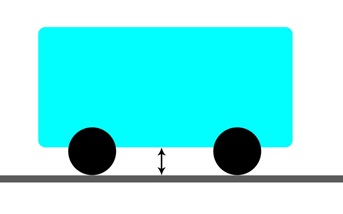
\includegraphics[width=0.92\linewidth]{chapters/chapter27/images/1}
		\caption{Дорожный просвет.}
		\label{ris:image27x1}
	\end{center}
\end{figure}

\begin{figure}[h!]
	\begin{center}
		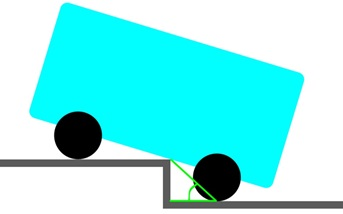
\includegraphics[width=1\linewidth]{chapters/chapter27/images/2}
		\caption{Угол продольной проходимости.}
		\label{ris:image27x2}
	\end{center}
\end{figure}	

Изначально в модели были использованы колёса диаметром 5 см. Затем они были заменены на большие, диаметром 10 см. В результате Дорожный просвет увеличился с 3 см до 6 см, а угол продольной проходимости – с \(20^\circ\) до \(30^\circ\). 

Также для большей устойчивости в середине корпуса было добавлено дополнительное колесо из шестерёнок диаметром 1,5 см. За счёт этого робот может преодолевать пригорки и ямы, не прогибаясь.\\
{\slshape Из наблюдений за командой известно, что у них происходили обсуждения конструкции корпуса (см. Занятие~\ref{lesson25}), но единственное место, где отражены хотя бы результаты~--- это полная модель робота, созданная в LDD по итогам четвертой недели.}

\begin{figure}[h!]
	\begin{center}
		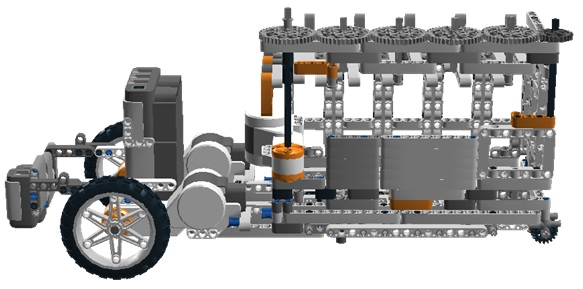
\includegraphics[width=1\linewidth]{chapters/chapter27/images/3}
		\caption{Вид со стороны дверей.}
		\label{ris:image27x3}
	\end{center}
\end{figure}

\begin{figure}[h!]
	\begin{minipage}[h!]{0.5\linewidth}
		\begin{center}
			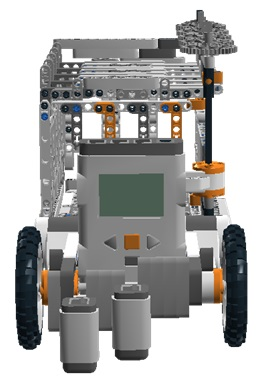
\includegraphics[width=1\linewidth]{chapters/chapter27/images/4}
			\caption{Вид спереди.}
			\label{ris:image27x4}
		\end{center}
	\end{minipage}
	\begin{minipage}[h!]{0.5\linewidth}
		\begin{center}
			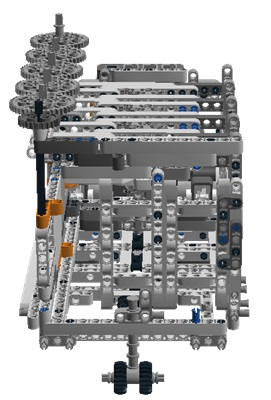
\includegraphics[width=1\linewidth]{chapters/chapter27/images/5}
			\caption{Вид сзади.}
			\label{ris:image27x5}
		\end{center}
	\end{minipage}
\end{figure}